\documentclass{ctexart}
\usepackage{indentfirst}
\usepackage{array}
\usepackage{graphicx}
\usepackage{url}
\graphicspath{ {images/} }
\begin{document}

\title{基于ARM架构的超低功耗OS调研报告}
\author{崔天一\ 曹焕琦\ 邓翔\ 李泽昌}
\date{\today}
\begin{abstract}
本文首先介绍了对于开发平台的选择,包括蓝牙芯片DA14580的简要介绍以及与相似蓝牙开发平台的对比分析,接着简要阐述了在使用DA14580蓝牙芯片的嵌入式单片机上移植实时操作系统的优势,包括最终所确定的操作系统µC/OS-II的优越性。最后介绍了目前在可穿穿戴设备上降低功耗的必要性,以及目前工业界拥有的成果,简述我们的解决方案的优势所在。
\end{abstract}

\maketitle

\tableofcontents
\newpage
\section{开发平台的选择}

对于开发平台的选择,我们需要同时考虑到低功耗特性和足够的功能以面对各类实际问题。下面我们比较一下若干可能选择的情况。
\begin{center}
\begin{tabular}{| m{10em} | m{5em} | m{2em} | m{9em} |}
\hline
平台类型 & 开发方式 & 功耗 & 功能 \\
\hline
FPGA & HDL & 极低 & 可强可弱,实现困难 \\
\hline
高效高通用性平台\par(如ARM Cortex-A) & 汇编语言,\par C/C++ & 较高 & 强 \\
\hline
高可靠性嵌入式平台\par(如ARM Cortex-R) & 汇编语言,\par C/C++ & 中 & 较强 \\
\hline
高能效嵌入式平台\par(如ARM Cortex-M) & 汇编语言,\par C/C++ & 低 & 较强 \\
\hline
\end{tabular}
\end{center}
由以上列表可看出,出于实现难度、功耗、功能三方面考虑,高能效的嵌入式平台更加适合超低功耗的可扩展平台的开发。基于此理由,我们倾向于选择高能效的微处理器。\par
\begin{figure}[h]
\centering
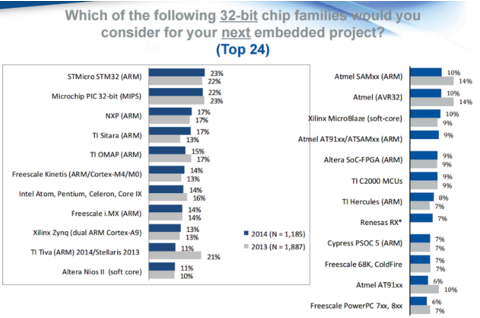
\includegraphics[scale=0.65]{cpu}\par
\end{figure}
在微处理器的架构选取中,主要有ARM、MIPS、AVR32、Intel Atom等架构。为方便开发,我们倾向于选取使用率较高的微处理器架构;因为它们的相关资料往往较多,开发难度也较低,同时使用率高也代表着它有着其独特的优越性。\par
在上图中,我们可以看到,ARM架构处理器占据了前五名的三个位置;由此可见ARM架构有着更加适合嵌入式开发的特性。我们倾向于选择ARM Cortex-M系列微处理器,它在硬件条件令人满意的同时,也有着丰富的开发资源和良好的生态环境,能够适应我们的高可扩展性要求。\par
而在比较Cortex-M系列各芯片中,Cortex-M0的功耗最低,虽然主频通常较低、功能也较弱,但在嵌入式的环境下已经足够使用。

\section{实际平台的选取——BLE芯片DA14580}

Bluetooth Smart,技术称Bluetooth low energy,在2006年由Nokia提出,并于2010年正式由SIG加入Bluetooth标准。它的主要目标是保证传输范围与效果的前提下,大幅度降低功耗。近年来,绝大多数移动平台,包括移动电话、笔记本电脑、可穿戴设备,均包含Bluetooth Smart支持;见下图。\par
\begin{figure}[h]
\centering
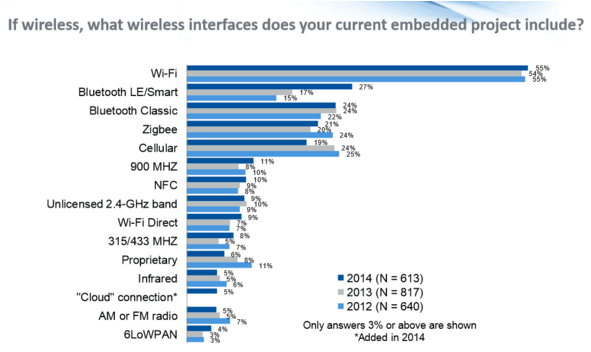
\includegraphics[scale=0.5]{bluetooth}\par
\end{figure}
从图中我们可以看出,除Wi-Fi由于其互联网链接特性有着比Bluetooth更高的占有率外,Bluetooth Smart在连续的飞速增长中占居第二,作为其前代产品的Bluetooth Classic也始终稳居前几名。蓝牙有着便利的数据传输功能,相比其它无线连接往往更低的功耗,和令人满意的速度;因此,以蓝牙为基底进行低功耗OS的开发是合理的,尤其是考虑到Bluetooth Smart本身的低功耗特性。
一方面Bluetooth Smart模块可作为复杂设备(如移动电话)的组件,另一方面也可以作为可穿戴设备等小型设备的中心组成;对于后一种情况,往往需要一个适用于嵌入式的低功耗CPU来完成整个系统。
这里我们比对流行的蓝牙智能芯片的数据如下\cite{da14580}\cite{cc2540}\cite{csr101x},休眠时保留时钟:
\begin{center}
\begin{tabular}{| c | c | c | c | c |}
\hline
芯片型号 & RX工作电流 & TX工作电流 & 休眠电流 & 处理器 \\
\hline
DA14580 & 4.9mA & 4.9mA & 400nA & ARM Cortex-M0 \\
\hline
CC2540 & >19.6mA & 24mA & 900nA & ARM Cortex-M0 \\
\hline
CSR101x & ~20/18mA & ~20/18mA & 5uA & 8051 \\
\hline
\end{tabular}
\end{center}
三类流行的蓝牙智能芯片之间,功耗对比十分明显:DA14580有着远低于其它二者的功耗。同时,搭载了ARM Cortex M0微处理器的DA14580也有着足够的灵活度以面对各种实际问题。综合各方面因素,它是低功耗高灵活度蓝牙智能平台解决方案的最佳选择之一,本项目中也将选择此芯片作为平台。

\section{单片机移植嵌入式操作系统优越性}

传统单片机通常并未安装操作系统,通过各类为特定目的编写专用程序来实现相应功能,在过去各类功能需求较为有限的情况下,这种方式能够提供足够可靠的解决方案。然而随着时代的发展却暴露出了越来越多的问题。 但是通过移植操作系统可以较好的解决这些问题,具体如下:\par
\begin{enumerate}
  \item 降低开发门槛。\par
    传统单片机应用的开发,通常与底层硬件紧密相关,这要求开发人员不仅需要掌握程序设计的一般技巧, 更要对于底层硬件语言与各类接口有着较好的理解,这大大提高了开发门槛, 使得只有极少数人能够为单片机开发应用。将操作系统 移植到单片机之后可以使各类开发者专注于自己的本职工作。软件开发者可以将注意力放在如何通过与操作配合开发出更加高效以及功能更加丰富的软件。而系统工程师则可以更多的关注于操作系统与硬件之间的协同,从而在性能和功耗之间达成更好的平衡。\cite{rtos}类似于编程语言从机器码到汇编到高级程序设计语言的进步。可以大大提高效率。
  \item 便于外设添加以及应用开发移植。\par
    传统方式的单片机开发在往往应用与硬件结合较为紧密,一旦软件编写结束烧入板子之后如果需要加入新的功能往往需要将原有的设计完全推翻重来,即使不必如此也往往会将原有的设计打乱,从而影响整体的工作效率。而移植操作系统之后,操作系统将底层接口等封装起来,从而大大提高了效率并缩减了所需要的时间,这在如今功能需求变化迅速的时代尤为重要。同时操作系统使得同一应用在不同平台之间的移植变得便利,减少了开发人员的负担,能够吸引更多人参与开发,促进产业发展。\cite{rtos_in_mcu}
  \item 便于纠错和分析。\par
    传统单片机开发软件编写好之后需要烧入芯片才能进行调试。调试需要使用专用接口并且需要有相应的开发经验和对于底层硬件很强的理解,非常不便和耗时。同时也很难区分究竟是硬件问题还是软件问题。当应用程序变得复杂之后,这些问题会越发的凸显出来。\par
    \begin{figure}[h]
\centering
    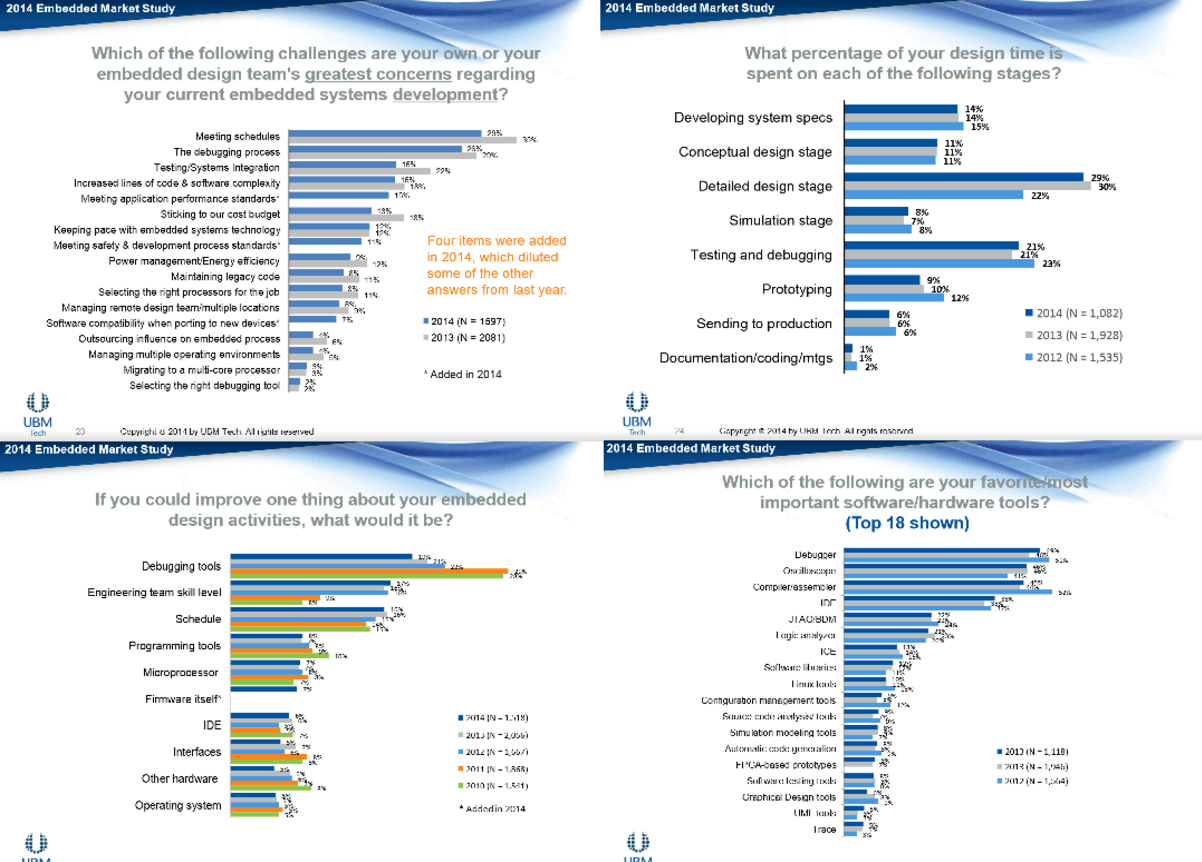
\includegraphics[scale=0.25]{debug}\par
    \end{figure}
    由以上调查可知\cite{survey},真实开发过程中,检错测试所占用的时间与开发耗时近乎相等。同时许多开发者也表示调试工具的便利性是他们非常重视的一个环节。而许多操作系统自带相关的调试和分析工具,能够帮助开发者迅速发现问题从而解决问题。同时,操作系统能够协助开发者检测应用的资源消耗,从而针对性的进行优化。
  \item 更出色的多任务调度。\par
    操作系统提供了更好并且更安全的多任务并行方式,在不含操作系统的小型单片机中,开发者常常利用全局变量来实现不同模块和应用间的通信和同步。但是大量使用全局变量可能导致错误与安全性问题,尤其是当系统规模变大时,这些被共享的信息很容易造成冲突从而影响系统整体的工作效率甚至导致系统崩溃。但是RTOS通常都已经提供了较为完善的进程调度方案,移植操作系统后,开发者便可以专注于应用本身的开发而将这些协调问题交给操作系统解决。
  \item 对于硬件资源的更加高效的应用。\par
    传统的单片机应用多采取轮询方式来检测中断是否发生,结果导致了大量的核心闲置时间。得益于多任务实时操作系统所采用的中断驱动方式,我们可以最大限度的减少轮询。这使得核心的资源得到了最大化利用,并且能够在闲置时尽可能多的进入休眠状态从而降低功耗。\cite{rtos_in_mcu}
\end{enumerate}

\section{嵌入式操作系统选择——µC/OS-II}

嵌入式操作系统是在嵌入式设备上运行的操作系统,这类系统通常具有紧密、高效、可靠、实时等特性。\cite{wiki01}这类操作系统通常为实时操作系统(RTOS),运行在资源受限的设备上,它们内存通常较少,且为了充分利用CPU,有一部分代码使用汇编语言编写。特别地,嵌入式操作系统区别于其他的桌面操作系统,通常不从ROM中动态加载应用程序,而是将所用应用程序和操作系统自身打包成一个刷写镜像刷写至设备中。\par
目前,市面上流行的嵌入式操作系统主要有以下几类:\cite{os}\par
\begin{itemize}
  \item 嵌入式Linux\cite{wiki02}\par
    这类操作系统以Linux内核为基础,被设计用来使用嵌入式设备,这类操作系统被广泛的用在手机等消费产品中。\par
    \begin{figure}[h]
\centering
    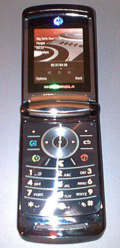
\includegraphics{mobilephone}\par
    \end{figure}
    如上图为一个使用了嵌入式Linux的手机。该系统和其他系统相比有以下好处:
    \begin{itemize}
      \item 开放源代码
      \item 不需版权费用
      \item 成熟与稳定(经过这些年的发展和使用)
    \end{itemize}
    但是,我们不能采用嵌入式Linux系统作为我们移植至芯片上的系统,这是因为一个RTLinux通产需要2M存储空间,但开发板上通产只有若干KB的存储空间(对于开发板来说是84KB),由于存储空间的限制,无法使用这类操作系统。
  \item Windows CE\cite{wiki03}\par
    Windows Embedded Compact(旧称Microsoft Windows CE)为微软研发的一套嵌入式操作系统,如下为Windows CE的发布历史。\par
    \begin{figure}[h]
\centering
    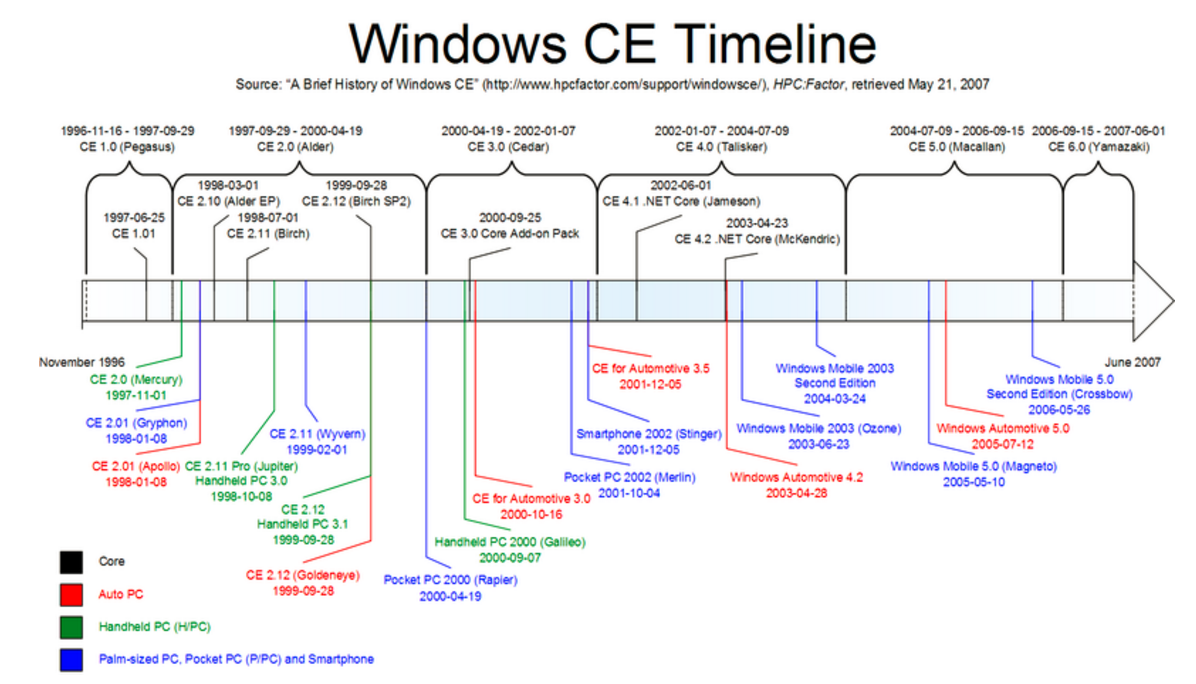
\includegraphics[scale=0.25]{wince}\par
    \end{figure}
    但我们仍然无法使用其作为我们要移植的操作系统,这是因为Windows CE未完全开放其源代码,使我们的移植工作受到了很大的限制。另外,Windows CE的实时性不如μC/OS。
  \item VxWorks\cite{wiki04}\par
    VxWorks是美国WindRiver公司设计的一种RTOS,具有高性能的内核、友善的开发环境,且有较高的市场份额。\cite{Turley_undated-jf}如下为各商业嵌入式操作系统的市场份额。且其广泛应用于通信、航空、航天、军事等领域内。特别是国内军用手持设备也大量的使用了Vxworks的产品。\par
    \begin{figure}[h]
\centering
    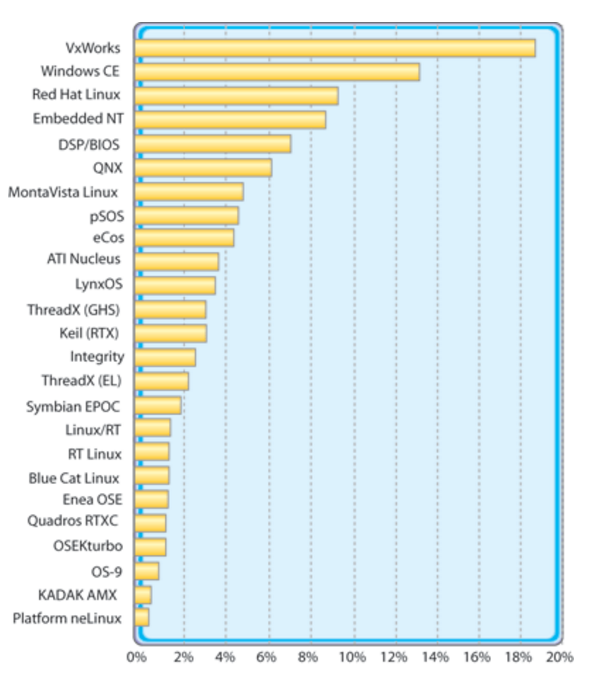
\includegraphics[scale=0.3]{vxworks}\par
    \end{figure}
    但使用其需要支付昂贵的授权费,故我们无法使用该操作系统。
  \item µC/OS-II\cite{wiki05}\par
    µC/OS-II是由Jean J. Labrosse于1991年开发的实时操作系统,它基本上是用C语言编写完成的,具有可固化、可移植的特性。其进程调度是根据优先级进行的。同时,该系统还提供了内存管理、时序管理(timing)、进程间通讯等功能。\par
    在本项目中,我们由于其源码可得、代码精简、可移植性强、文档丰富的特性选择其为我们带移植的系统。
  \item µC/OS-III\cite{noauthor_undated-vf}\par
    µC/OS-III系统为2009年发布的针对µC/OS-II的改进版本,其主要增加了如下的功能
    \begin{itemize}
      \item Round robin进程调度算法
      \item 将进程数上限由255提升至无限
      \item 允许多进程共享相同的优先级
    \end{itemize}
    但由于µC/OS-III的代码长度和复杂程度比µC/OS-II有一定程度的增加,为了保证项目的结构和代码的清晰,同时考虑到在我们的平台上进程数较少,µC/OS-III更加优秀的进程调度可能没有显著的效果,我们使用µC/OS-II作为待移植的系统而非µC/OS-III。
\end{itemize}

\section{µC/OS-II的优点}

\begin{enumerate}
  \item 可移植\par
    µC/OS-II源代码公开且绝大多数用ANSI C编写,其余用较少量的汇编语言编写,可分为内核层和移植层,因此移植起来比较方便。只要对应的微处理器具有堆栈指针和CPU内部出栈、入栈指令,µC/OS-II就可以移植,故现已广泛用于8位、16位和32位甚至64位的单片机或DSP。
  \item 可裁剪\par
    可以根据用户的需求,选择性地减少µC/OS-II的调用,以此减小存储器的占用。而且可裁剪性可以通过条件编译较为简易地进行实现。充分裁剪后的µC/OS-II系统可以达到10K以内,故认为其满足嵌入式系统的要求。
  \item 可固化\par
    µC/OS-II专门为了嵌入式系统而设计,只要具备合适的系列软件工具(C编译、汇编、链接及下载/固化),完全可以将µC/OS-II嵌入到产品中。
  \item 稳定性\par
    2000年7月,µC/OS-II得到了FAA对用于商用飞机、符合RTCA DO-178B标准的认证。这个认证充分说明了µC/OS-II的安全性与稳定性,能用于像商业飞机这样苛求安全稳定的场合。
  \item 系统服务\par
    µC/OS-II提供了许多系统服务,如信号量、事件标志、消息队列、消息邮箱等等。
\end{enumerate}

\section{µC/OS-II的应用}

µC/OS-II由于其可靠性、轻量性,被广泛地应用于各类特殊用途的嵌入式开发。在以下嵌入式系统中,有大量的产品选择使用了µC/OS-II。
\begin{itemize}
  \item Avionics
  \item Medical equipment/devices
  \item Data communications equipment
  \item White goods (appliances)
  \item Mobile phones, PDAs, MIDs
  \item Industrial controls
  \item Consumer electronics
  \item Automotive
\end{itemize}
这里我们列举一些实际的应用。
\begin{itemize}
  \item 好奇号火星车\par
    好奇号火星车上搭载的用来探测火星大气与土壤中化学与同位素成分的SAM模块是由µC/OS-II操作系统内核控制的。它的高实时性保证了配合采集行为即时分析物质组成的能力,它的高可靠性同时保证了组件在恶劣环境下的正常工作。\par
    \begin{figure}[h]
\centering
    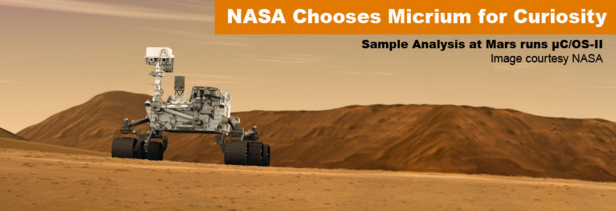
\includegraphics[scale=0.5]{curiosity}
    \end{figure}
  \item 基于µC/OS-II和MSP430F5438A的心率监视仪\par
    Texas Instruments推出的MSP430F5438A可用于制造心率监视仪。根据来自TI的应用报告,他们推荐使用µC/OS-II作为平台来进行开发。这说明了µC/OS-II的高可靠性,同样也侧面表明了µC/OS-II的广泛用途。\par
    \begin{figure}[h]
\centering
    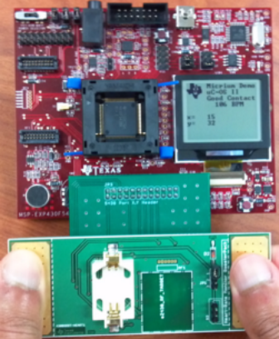
\includegraphics[scale=0.5]{heart}
    \end{figure}
\end{itemize}

\section{µC/OS-II部分特性简介}

\begin{enumerate}
  \item 任务管理\par
    µC/OS-II可以管理多达64个任务,每个任务的优先级均不同,故µC/OS-II有64个优先级,级号越低,优先级越高。例如当µC/OS-II初始化时,优先级最低的OS\_LOWEST\_PRIO总被赋与空闲任务idle task。因为优先级是唯一的,故µC/OS-II也可通过优先级来识别任务。由于保留8个优先级,用户有多达56个应用任务。每个任务放在任务就绪表中,里面有两个变量OSRdyGrp和OSRdyTbl[]。可以任务的就绪状态通过这两个变量的置位来表示。
  \item 内存管理\par
    malloc和free这两个函数在ANSI C中被用来动态控制内存的分配与回收。但在嵌入式操作系统中,这样做却是十分危险的。如果多次地调用这两个函数,原本一块完整的较大的内存区域会被分割成许多不相邻且非常小的内存碎片。最终程序将连一块很小的内存也申请不到。µC/OS-II 通过把内存分区管理,解决了这个问题。每个区包含整数个大小相同的内存块。于是,µC/OS-II改进了malloc和free两个函数,使之申请与释放固定大小的内存块。如图所示,不同的分区的内存块大小不同,于是通过申请不同分区的内存块,可获得不同大小的内存,释放时同样回到原内存分区。\par
    \begin{figure}[h]
\centering
    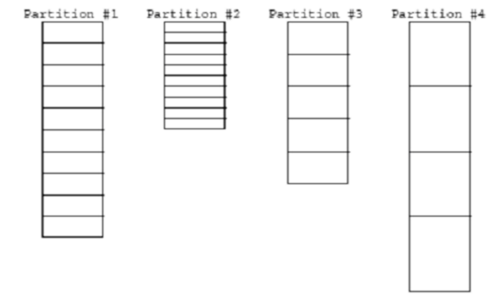
\includegraphics[scale=0.4]{memory}
    \end{figure}
  \item 时间管理\par
    µC/OS-II要求提供定时中断,以实现延时与超时等功能。用硬件定时器产生一个周期为ms级的周期性中断来实现系统时钟,最小的时钟单位就是两次中断之间相间隔的时间,这个最小时钟单位叫做时钟节拍(Time Tick),应发生10-100次/秒。时钟节拍的频率越高,系统负荷越大。硬件定时器以时钟节拍为周期定时地产生中断,该中断的中断服务程序叫做OSTickISR()。中断服务程序通过调用函数OSTimeTick()在每个时钟节拍了解每个任务的延时状态,使其中已经到了延时时限的非挂起任务进入就绪状态。有时需要让高优先级的任务暂时让出CPU的使用权,那么可以用OSTimeDly()函数暂停当前任务的运行。此外还有取消延时的OSTimeDlyResume()函数,获取系统时间的OSTimeGet()函数等等。总而言之,µC/OS-II对时间的操作是非常灵活的。
  \item 互斥型信号量\par
    µC/OS-II是可剥夺性内核,当任务以独占方式使用共享资源时,会出现任务优先级反转的情况。下图显示的就是从t1到t6出现的优先级反转情况。为了解决这个问题,应让获得信号量正在使用共享资源的优先级暂时得到提升,要高于所有任务,从而使共享资源尽快被使用完而释放。等释放了信号量,再恢复任务原有的优先级。而互斥型信号量的ECB模型就支持临时提升优先级的操作。\par
    \begin{figure}[h]
\centering
    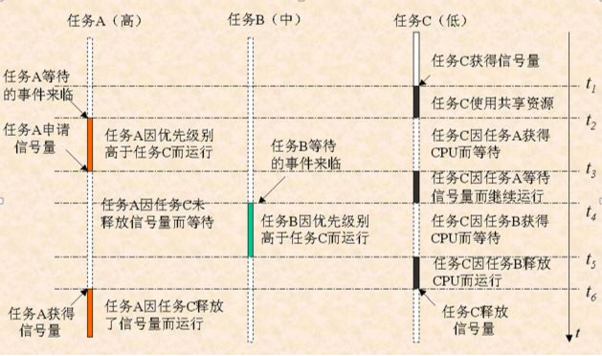
\includegraphics[scale=0.4]{preempt}
    \end{figure}
\end{enumerate}

\section{降低芯片功耗的必要性}

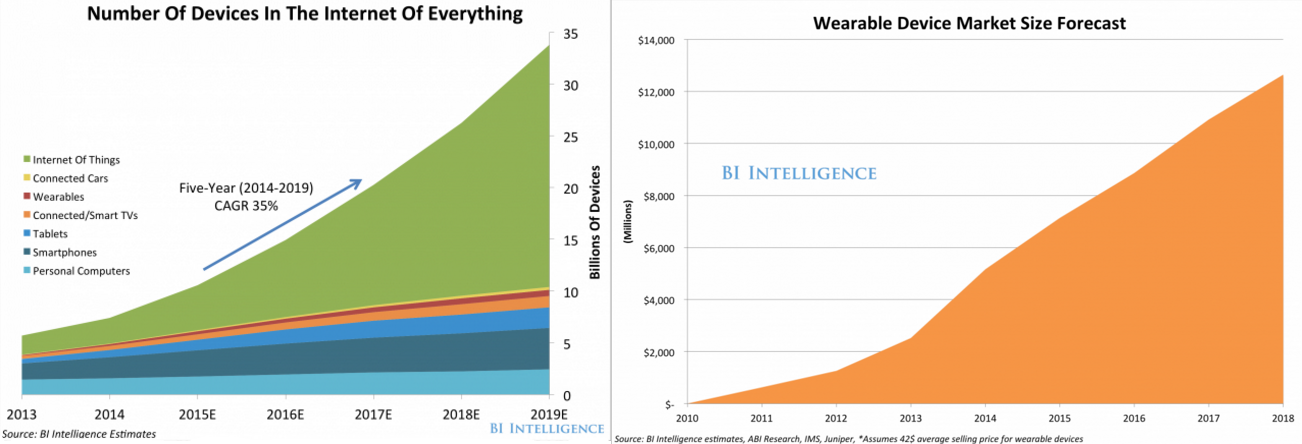
\includegraphics[scale=0.25]{market}\par
从上二图中可以看到,随着互联网技术的发展,物联网、智能家居、可穿戴设备也进入了人们的视野。\cite{Ballve2013-bp}而作为新时代中新的人机交互形式和更便利的电子设备,可穿戴设备的市场预期也在不断地增长,各大厂商亦在不断地推出新产品。\cite{noauthor_2015-cg}但由于可穿戴设备的低重量、小体积要求,它们往往只能配备小容量电池;为了保证待机,必须做到较低的功耗。\par
\begin{figure}[h]
\centering
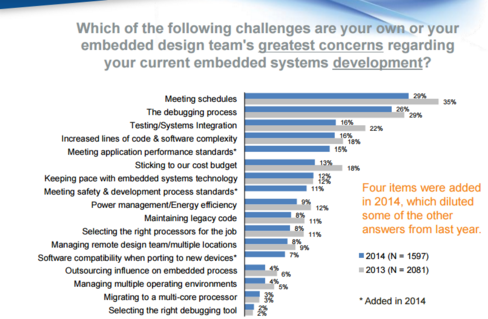
\includegraphics[scale=0.5]{power}\par
\end{figure}
在上图中\cite{survey},我们可以发现,降低芯片功耗的必要性已经纳入了许多开发者最优先考虑的因素;功耗决定待机时间,而待机时间极大地影响着产品在市场上的受欢迎程度。\par
但同时,我们需要注意到,通常的嵌入式开发由于往往出于种种因素不考虑通用性,也即并不存在完整的操作系统,因而能够避免CPU调度、完整地调配CPU的行为,在适当的时候进行休眠,从而避免功耗的增加;但当我们为了通用性和可扩展性而加入操作系统时,功耗就变得很难以降低。对于通常的操作系统,CPU始终工作,导致了巨大的能耗;同时,若不适时地关闭蓝牙模块,它的功耗也是不能忽视的。

\section{休眠——一种降低功耗的实现}

ARM Cortex-M0微处理器允许芯片制造商提供了多种能耗模式(Energy Mode)进行选择,这是指关闭或开启部分组件从而在牺牲一部分功能的情况下降低功耗。如下图为某芯片提供的在各个能耗模式间切换的状态图:\par
\begin{figure}[h]
\centering
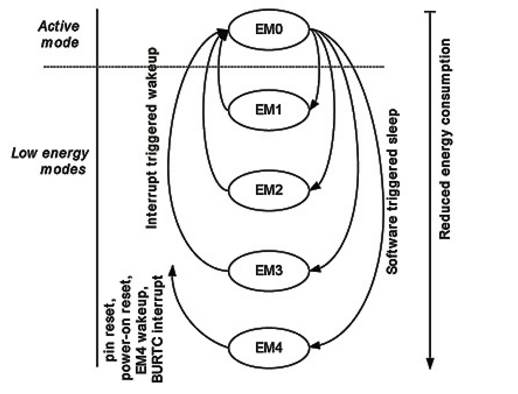
\includegraphics[scale=0.5]{sleep}\par
\end{figure}
如上图所示,该芯片正常工作在EM0,当执行相应的休眠指令时,会转移至相应的休眠状态(EM1~4)。对于EM1~3,可通过中断唤醒;对于EM4,只能通过外部Reset信号唤醒。休眠状态的数量和行为并不由ARM定义,而是由芯片制造商定义。\par
\begin{figure}[h]
\centering
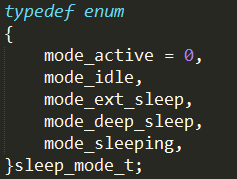
\includegraphics[scale=0.5]{sleep_mode}\par
\end{figure}
根据上图(来自Dialog提供的DA14580 SDK),对于DA14580,它将四种休眠状态缩减为3种:Idle,Extended Sleep Mode和Deep Sleep Mode。对于第一种和第二种,它们通过中断唤醒,类似于先前的芯片的EM1~3;对于后者,它通过特定信号唤醒,相当于EM4。在Idle状态下,芯片中的CPU停止工作,但蓝牙保持工作状态,SysRAM上电;在Extended Sleep Mode中,处理器和蓝牙休眠,但保持SysRAM上电;在Deep Sleep Mode中,处理器、蓝牙和SysRAM均停止工作。mode\_sleeping指将进入休眠,具体休眠状态由应用决定。\par
在大多数现有的通用系统中,由于CPU性能往往过剩,CPU处于等待任务状态的时间往往较长。若按照传统方案,Idle状态CPU应处在一个循环中,直到新任务抵达。但在这个循环中,CPU将进行大量的取指、译码、执行等操作,大幅度提高了功耗。如下图,在Windows NT内核操作系统中,System Idle Process往往占用着超过90\%的CPU时间\cite{wiki06}。\par
\begin{figure}[h]
\centering
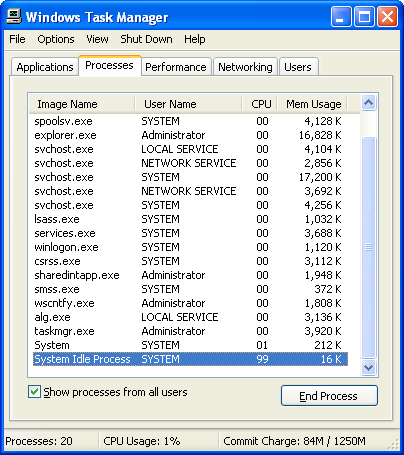
\includegraphics[scale=0.5]{idle}\par
\end{figure}
因此,可以考虑将Idle循环替换为休眠,以实现功耗的降低。而对应于µC/OS-II,在操作系统系统初始化后会建立一个优先级最低的任务——空闲任务。在没有任何任务就绪时会执行这个空闲任务,即进入idle任务。\par
如下图所示,在task3执行完毕后,执行task2之前,并不需要频繁地唤醒系统。若在tick8处唤醒系统,系统仍然会进入idle任务。因此可利用µC/OS-II的空闲任务扩展接口,进入低功耗模式而不影响其他任务的调度与系统的稳定性,降低系统的功耗。与此同时,利用RTI信号周期性地唤醒CPU。系统被唤醒后,将执行中断服务程序,做一定的处理后,检测当前是否有任务恰好处于就绪态。若存在任务处于就绪态,则执行该任务,否则重复上述的操作。这也是当下流行的µC/OS-II低功耗处理方法。\par
\begin{figure}[h]
\centering
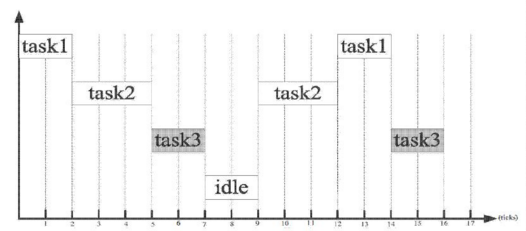
\includegraphics[scale=0.5]{ucos_idle}\par
\end{figure}
而关于具体的实现,一种实现方法是,首先在进入idle任务时遍历当前任务链表,获取所有等待状态任务的最小延时。再把定时器设为这个时间,由此便可以增加进入低功耗模式的时间,减少唤醒次数,降低系统的功耗。经过这段最小延时后,触发中断服务程序。该中断服务程序将当前系统的基时加上该最小延时,遍历任务链表,把任务的等待时间减去该最小延时,此时应有任务处于就绪状态,最后中断服务程序退出。在idle任务时查找最小延时需要临时关闭中断,等待被定时器唤醒时,开中断,执行终端服务程序。\par
再回到DA14580。考虑到蓝牙模块的能耗,在idle任务下不仅需进入mode\_idle,还需适当地关闭蓝牙模块,即进入mode\_ext\_sleep。通过这样的处理,我们能够大幅度地降低功耗。由于现有的低能耗解决方案往往没有出现在带有蓝牙功能的芯片上,适时关闭蓝牙模块的方式与效果尚需要我们进行研究与完成其实现。\par

\section{结论}

随着技术发展与市场扩张,低功耗高可用的小型设备的重要性变得不可忽视。而以低功耗、高可用性、高可扩展性为目标,我们选定了基于ARM架构的DA14580芯片,并将在其上移植µC/OS-II,进而实现休眠式的Idle,以完成超低功耗的目标。\par

\bibliography{main.bib}
\bibliographystyle{plain}
\end{document}
